\subsection{Totale Ore}

\subsubsection{Totale suddivisione ore}
Di seguito è riportato il totale delle ore rendicontate:

\renewcommand{\arraystretch}{1.5}
\begin{table}[H]
\begin{center}
\begin{tabular}{|c|c|c|c|c|c|c|c|}
\hline
\rowcolor{title_row}
\textbf{\color{title_text}{Nome}} & \textbf{\color{title_text}{Resp.}} & \textbf{\color{title_text}{Ammi.}} & \textbf{\color{title_text}{Analist.}} & \textbf{\color{title_text}{Progett.}} & \textbf{\color{title_text}{Program.}} & \textbf{\color{title_text}{Verific.}} & \textbf{\color{title_text}{Totale}} \\ \hline
Andrea Trevisin  & & 14 & & 24 & 32 & 35 & 105  \\ \hline
Giacomo Barzon   & 4 & 9 & & 28 & 33 & 31 & 105  \\ \hline
Giovanni Sorice  & 14 & 8 & & 22 & 32 & 29 & 105 \\ \hline
Lorenzo Busin    & 7 & 6 & & 25 & 34 & 33 & 105 \\ \hline
Marco Costantino & 6 & 7 & 5 & 14 & 37 & 36 & 105 \\ \hline
Michele Roverato & & 10 & 8 & 18 & 37 & 32 & 105 \\ \hline
Nicolò Tartaggia & 10 & 5 & 13 & 16 & 36 & 25 & 105  \\ \hline
\end{tabular}
\caption{Tabella 5.6.1: Distribuzione oraria totale\label{}}
\end{center}
\end{table}
\renewcommand{\arraystretch}{1}

Il seguente grafico dà una rappresentazione visiva della suddivisione oraria: \\
\begin{figure} [H]
	\centering
	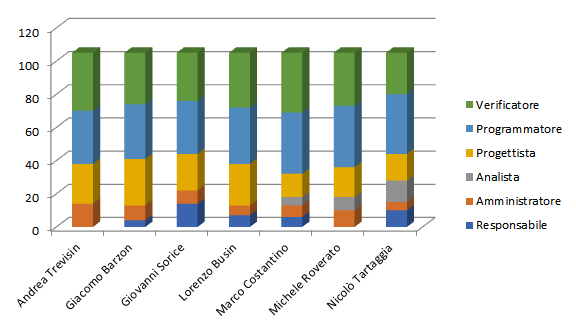
\includegraphics[scale=1]{Res/ExcelGrafici/Grafici/TotaleOre.png}
	\caption{Figura 5.6.1: Grafico suddivisione oraria totale delle ore tra i componenti del gruppo}\label{}
\end{figure}

\subsubsection{Totale Prospetto Economico}
Di seguito è riportato il totale delle ore dei diversi ruoli del progetto contando solo le ore rendicontate:

\renewcommand{\arraystretch}{1.5}
\begin{table}[H]
\begin{center}
\begin{tabular}{|c|c|c|}
\hline
\rowcolor{title_row}
\textbf{\color{title_text}{Ruolo}}  & \textbf{\color{title_text}{Ore}} & \textbf{\color{title_text}{Costo in \euro}} \\ \hline
Responsabile    & 41 & 1.230  \\ \hline
Amministratore  & 59 & 1.180 \\ \hline
Analista        & 26 & 650 \\ \hline
Progettista     & 147 & 3.234 \\ \hline
Programmatore   & 241 & 3.615 \\ \hline
Verificatore    & 221 & 3.315 \\ \hline
\textbf{Totale} & \textbf{735}    & \textbf{13.224}           \\ \hline
\end{tabular}
\caption{Tabella 5.6.2: Prospetto economico del totale delle ore rendicontate\label{}}
\end{center}
\end{table}
\renewcommand{\arraystretch}{1}

Il seguente grafico dà una rappresentazione visiva della distribuzione dei ruoli: \\
\begin{figure} [H]
	\centering
	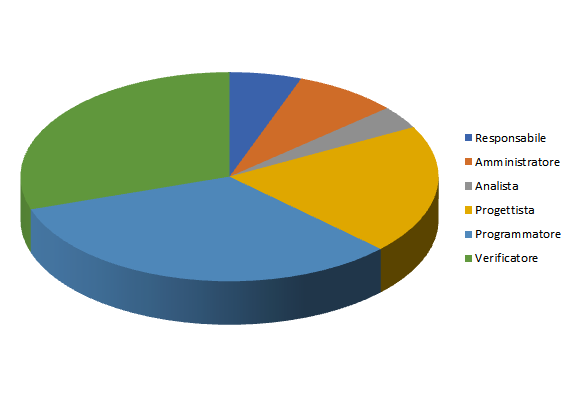
\includegraphics[scale=1]{Res/ExcelGrafici/Grafici/TotaleRuoli.png}
	\caption{Figura 5.6.2: Grafico suddivisione oraria totale di ogni ruolo}\label{}
\end{figure}


\pagebreak
